\chapter{Scelta Tecnologica}
\label{chap:scelta}
In questo capitolo viene trattata l'architettura utilizzata per unicam-product-editor e il modo in cui vengono gestiti i dati attraverso la web app, per poi passare ad illustrare l'organizzazione del codice.

Per sviluppare unicam-product-editor è stato utilizzato lo stack MEAN\index{MEAN} che non è altro che l'insieme dei quattro componenti che ne fanno parte:
\begin{itemize}
	\item M = MongoDB: il popolare database
	\item E = Express.js: un framework web leggero
	\item A = Angular.js: un framework per la creazione di single page application
	\item N = Node.js v4: un interprete JavaScript costruito sul motore JavaScript V8 di Google Chrome orientato agli eventi che lo rende efficiente e leggero
\end{itemize}
Lo stack MEAN è un' alternativa al più tradizionale stack LAMP\index{LAMP} (Linux, Apache, MySQL, PHP/Perl/Python/P…), molto popolare per il suo utilizzo nella costruzione di applicazioni web dagli anni '90 in poi.
Di seguito andiamo a costruire le RESTful API, che sono la base per qualsiasi tipo di applicazione, come un sito web, un'app Android, iOS o Ubuntu Touch.

\section{Oggetti 3D}
Un modello 3D è una rappresentazione matematica di un oggetto tridimensionale e consiste sostanzialmente in un file di dati strutturati, contenenti le proprietà delle primitive geometriche che costituiscono l'oggetto rappresentato (un corpo fisico). Un oggetto 3D quindi non è altro che un insieme di dati composto da punti nello spazio tridimensionale (tre dimensioni X, Y e Z) e altre informazioni (spesso metadati, o informazioni aggiuntive).
I principali formati utilizzati per i modelli 3D:
\begin{itemize}
	\item OBJ
	\item FBX
	\item Collada
	\item BLEND
	\item DFX
	\item STL
	\item PLY
	\item 3DS (obsoleto)
	\item VRML (obsoleto)
	\item X3D
\end{itemize}
La scelta per cui abbiamo optato per la realizzazione del nostro progetto è ricaduta sul .obj, o più correttamente Wavefront .obj\index{obj}, un formato di file sviluppato dalla Wavefront Technologies per il software Advanced Visualizer. Il motivo di questa scelta risiede nel fatto che il .obj è un formato aperto che è stato adottato da tantissimi applicativi per la grafica 3D per l'interscambio di dati con altri programmi; ciò lo rende perfetto per il nostro progetto, in quanto questo dovrà poi essere trasformato in un corrispondente file .JSON per poter essere interpretato dal viewer\index{unicam-product-viewer}.

Questo è, per intero, il file .obj per la creazione di un cubo

\begin{lstlisting}[caption={Cube.obj}, style=JavaScriptCode]
# cube.obj
#

g cube

v  0.0  0.0  0.0
v  0.0  0.0  1.0
v  0.0  1.0  0.0
v  0.0  1.0  1.0
v  1.0  0.0  0.0
v  1.0  0.0  1.0
v  1.0  1.0  0.0
v  1.0  1.0  1.0

vn  0.0  0.0  1.0
vn  0.0  0.0 -1.0
vn  0.0  1.0  0.0
vn  0.0 -1.0  0.0
vn  1.0  0.0  0.0
vn -1.0  0.0  0.0

f  1//2  7//2  5//2
f  1//2  3//2  7//2 
f  1//6  4//6  3//6 
f  1//6  2//6  4//6 
f  3//3  8//3  7//3 
f  3//3  4//3  8//3 
f  5//5  7//5  8//5 
f  5//5  8//5  6//5 
f  1//4  5//4  6//4 
f  1//4  6//4  2//4 
f  2//1  6//1  8//1 
f  2//1  8//1  4//1 
\end{lstlisting}
in cui sono specificate le posizioni e le grandezze nello spazio tridimensionale dei vertici (v), dei vertici normali (vn), e delle facce (f).

\newpage
L'oggetto 3D che ne deriva può essere facilmente visualizzato tramite ad esempio il programma Paint 3D:

\begin{figure}[h]
	\centering
	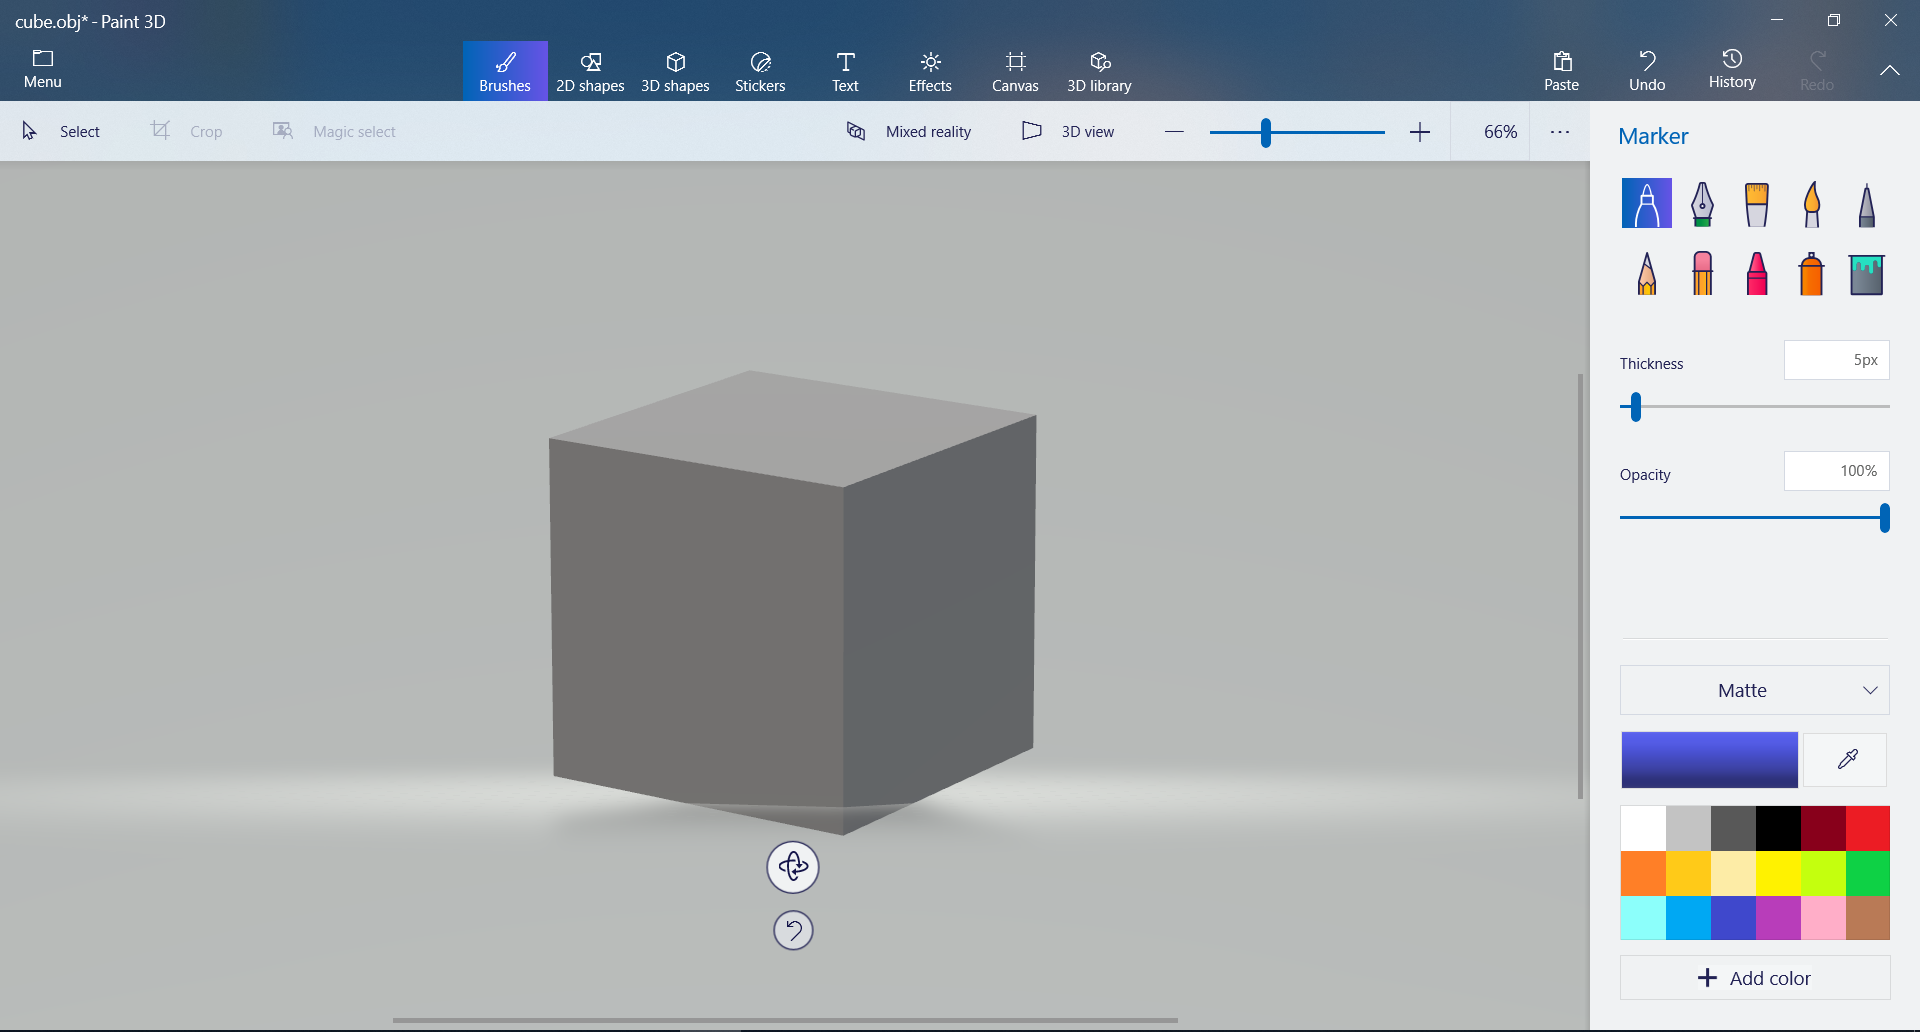
\includegraphics[scale=0.35]{Immagini/cube_obj.png}
	\caption{Visualizzazione grafica di cube.obj}
\end{figure}

\section{JSON}
JSON è un formato di dati molto leggere basato su un sottoinsieme della sintassi JavaScript, cioè \emph{array literal} e \emph{object literal}, proposto da Douglas Crockford come formato per i servizi web in sostituzione al verboso XML\index{XML}.

Dato l'utilizzo della sintassi Javascript, le definizioni JSON\index{JSON} possono essere incluse all'interno dei file JavaScript\index{JavaScript}.
\subsection{Gli array literal}

Gli \emph{array literal} rappresentano il metodo più semplice per creare un array in JavaScript.
Basta infatti elencare una insieme di valori separati da una virgola all'interno delle parentesi quadre, per esempio:
\begin{lstlisting}[style=JavaScriptCode]
var users = ["Paolo", "Antonio", "Filippo"];
\end{lstlisting}
A livello di programmazione è equivalente al codice:
\begin{lstlisting}[style=JavaScriptCode]
var users = new Array("Paolo", "Antonio", "Filippo");
\end{lstlisting}
Entrambe le definizioni generano lo stesso risultato ed è possibile accedere ad ogni elemento dell'array utilizzando il relativo indice 
\begin{lstlisting}[style=JavaScriptCode]
console.log(users[0]); \\prints Paolo 
console.log(users[1]); \\prints Antonio
console.log(users[2]); \\prints Filippo
\end{lstlisting}
Gli array in JavaScript hanno però due caratteristiche ben precise:
\begin{enumerate}
	\item In JavaScript l'array non ha un tipo di dati ben definito (non è tipizzato), e quindi ogni elemento può contenere tipi di dati diversi.
	\item Nonostante entrambi i metodi sopra citati per la creazione di un array siano validi in JavaScript, in .JSON soltanto gli array literal verranno accettati e interpretati correttamente.
\end{enumerate}

\subsection{Gli object literal}
Un object literal è definito tra parentesi graffe.
Al suo interno troviamo un numero qualsiasi di coppie chiave-valore, definite con una stringa, i due punti ed il valore.
Ogni coppia deve essere seguita da una virgola, tranne l'ultima. 
Questo insieme di coppie chiave-valore rappresenta, nel suo insieme, un oggetto.
Un esempio:
\begin{lstlisting}[style=JavaScriptCode]
var user = {
"firstname": "Paolo",
"age": 23,
"student": true
};
\end{lstlisting}
Il codice qui sopra genera un oggetto \emph{user} con le proprietà firstname, age e student. 
Per accedere alle proprietà dell'oggetto basta usare la notazione con il punto:
\begin{lstlisting}[style=JavaScriptCode]
console.log(user.firstname); \\prints "Paolo"
console.log(user.age); \\prints "23"
console.log(user.student); \\prints "true"
\end{lstlisting}
Lo stesso oggetto potrebbe essere creato utilizzando il costruttore \texttt{Object} di JavaScript
\begin{lstlisting}[style=JavaScriptCode]
var user = new object():
user.firstname = "Paolo";
user.age = 23;
user.student = true;
\end{lstlisting}
Come già detto, sebbene entrambe le definizioni siano accettate in JavaScript, in JSON è valida solo la seconda notazione, object literal.
\subsection{La sintassi JSON}
La sintassi di JSON non è altro che il miscuglio di object literal ed array literal per memorizzare dati e solo e soltanto rappresentarli.
Un esempio:
\begin{lstlisting}[style=JavaScriptCode]
[
{
"firstname": "Paolo",
"age": 23,
"student": true
},
{
"firstname": "Giuseppe",
"age": 40,
"student": false
}
]
\end{lstlisting}
La prima cosa da notare è che in questo documento non sono presenti variabili, così come punti e virgola.
In questo modo quando si trasmettono dei dati tramite HTTP ad un browser, il tutto avviene abbastanza velocemente grazie al numero ridotto di caratteri.

Oltre a questo, ci sono altri ovvi benefici nell'utilizzo di JSON come formato dati per la comunicazione in JavaScript: non bisogna preoccuparsi della valutazione dei dati, e quindi, è garantito un accesso più veloce alle informazioni che questo contiene.



\section{RESTful API}
Il significato dell’acronimo REST è REpresentational State Transfer, ossia una rappresentazione del trasferimento di stato di un determinato dato.

REST utilizza un modello client-server, dove il server è un server HTTP e il client invia richieste HTTP (GET, POST, PUT, DELETE), con un URL che al suo interno contiene i parametri codificati. L'URL descrive l'oggetto e il server genericamente risponde restituendo un'immagine, un documento HTML, un file CSV o qualunque altro tipo di dato.
Nel nostro caso il server risponde restituendo del codice e un JSON (JavaScript Object Notation).
Una RESTful API quindi è l'Interfaccia di Programmazione di un'Applicazione che usa le richieste HTTP per gestire i dati che vengono scambiati fra client e server.

Dato che in unicam-product-editor viene utilizzato lo stack MEAN, abbiamo scelto di utilizzare documenti JSON che risultano particolarmente adatti per la nostra applicazione, visto che tutti i nostri componenti sono in JavaScript e MongoDB interagisce perfettamente con questo formato. 
Faremo degli esempi più dettagliati più avanti quando definiremo i nostri Data Model.

Le operazioni principali che si possono eseguire con questo metodo sono le seguenti:
\begin{itemize}
	\item\texttt{GET} per richiedere al server un determinato set di dati;
	\item\texttt{POST} per creare un nuovo documento all’interno del database;
	\item\texttt{PUT} per modificare o sostituire completamente un documento già esistente;
	\item\texttt{DELETE} per cancellare un documento contenuto all’interno del database al quale siamo collegati. 
\end{itemize}

Queste operazioni vengono spesso descritte attraverso l'acronimo CRUD, che sta per CREATE, READ, UPDATE e DELETE.
Il server HTTP, da parte sua, usa spesso assieme alle API REST dei codici di risposta; di seguito vengono elencati alcuni fra i più comuni:
\begin{itemize}
	\item 200 - “OK”
	\item 201 - “Created” (Utilizzato con POST)
	\item 400 - “Bad Request” (Ad esempio per l'assenza di parametri)
	\item 401 - “Unauthorized” (Non ci sono i parametri per l'autenticazione)
	\item 403 - “Forbidden” (L'utente è autenticato ma non ha i permessi)
	\item 404 - “Not Found”
\end{itemize}
Una descrizione completa è contenuta nell'apposito RFC 2616\cite{RFC2616}.

Lo sviluppo di API REST è alla base del nostro sviluppo, in quanto permette alla nostra applicazione di essere multipiattaforma. Per fare alcuni esempi di applicazioni di questo tipo si possono citare Google Docs, Pixlr o lo stesso Trello insieme ad Evernote. Le API REST permettono la facile implementazione dell'applicazione su molte piattaforme che potranno essere sviluppate in un secondo momento, trasformando il progetto iniziale in un progetto indipendente dalla piattaforma di partenza.

I dati da gestire nel nostro progetto si possono riassumere in questo modo:
\begin{itemize}
	\item Dati degli utenti
	\item Liste
	\item Oggetti
	\item Opzioni di ogni oggetto
	\item Parti di ogni opzione
\end{itemize}
Come potremo vedere a breve, diversamente dai tradizionali Database relazionali (in cui la forma principale di struttura dati è data dalle Tabelle), in MongoDB, essendo un Database NoSQL, e quindi non relazionale, non si parla di Tabelle, anche se il concetto di Database ad alto livello è lo stesso.

Nel Database MongoDB possono essere contenute più Collection, che possono forse essere paragonate alle Tabelle nei Database relazionali. A sua volta, ogni Collection conterrà uno o più Document, che a confronto con un Database relazionale corrisponde all'incirca alla riga di una Tabella. Ogni Document (così come ogni Collection) non segue però uno schema specifico come in una Tabella, ma può essere formato da una o più coppie chiave-valore, dove il contenuto può essere a sua volta una variabile semplice oppure qualcosa di più complicato come un array.

Il documento JSON appena preso in esempio rappresenta un utente nel nostro sistema. Ogni campo ha il suo specifico scopo, ma il campo più importante in un Document MongoDB è senza dubbio il campo \texttt{\_id}: questo rappresenta la chiave primaria di ogni Document. Quando un Document viene salvato senza questo campo, MongoDB ne assegna uno automaticamente, e con un valore univoco.

Ora passiamo ai vari Document che compongono le nostre Collection; la Collection degli Utenti conterrà Documenti di questo tipo:
\begin{lstlisting}[caption={User Collection}, style=javaScriptCode]
{
	"_id": {
		"$oid": "5894fa05f882a91c7c5cf0e6"
	},
	"displayName": "Paolo Andreassi",
	"email": "pablo15941@gmail.com",
	"password": "$2a$10$kyaJc1WP9KFvSVWzrPagLe.vgY76FjBQjwt76.HhC5u9oo96qoRo.",
	"__v": 0,
	"picture": "https://graph.facebook.com/v2.3/10209758034881202/...",
	"google": "106815394034042298036"
}
\end{lstlisting}
Si può notare l'importante presenza del campo \texttt{\_id}, così come gli altri dati utili al riconoscimento dell'utente. La password inoltre in unicam-product-editor non viene mai mostrata in chiaro all'interno del Database, anche se il campo ad essa corrispondente è presente e popolato. Questo è il risultato di una password impostata dall'utente ma successivamente encriptata con una funzione hash.
\newpage
Il Document di tipo Lista ha uno scopo puramente descrittivo nei confronti di ciò che contiene:
\begin{lstlisting}[caption={List Collection}, style=javaScriptCode]
{
"_id": {
"$oid": "589a30d1b2a4c717a8da16b3"
},
"nome": "Omino LEGO",
"__v": 0
}
\end{lstlisting}

La Collection degli Oggetti avrà dei Document in cui i campi \texttt{nome} e \texttt{descrizione} hanno una funzione descrittiva, ma oltre al campo \texttt{\_id} è presente il campo \texttt{\_list} che funge da collegamento con la Collection delle Liste: in questo campo infatti è indicato l'identificativo della Lista a cui appartiene uno specifico Oggetto:
\begin{lstlisting}[caption={Object Collection}, style=javaScriptCode]
{
"_id": {
"$oid": "589a38f93ec83413e4f010b2"
},
"nome": "Omino LEGO",
"descrizione": "LEGO figure",
"_list": [
"589a30d1b2a4c717a8da16b3"
],
"__v": 0
}
\end{lstlisting}

Essendo un Database con una struttura nidificata, anche i Document nelle Collection delle Parti e delle Opzioni avranno una struttura simile a quelli delle Collection degli Oggetti: anche in queste infatti è indicato il campo del Documento \emph{parente} a cui fanno riferimento:
\begin{lstlisting}[caption={Part Collection}, style=javaScriptCode]
{
"_id": {
"$oid": "589a3a2857ba982460b83fb7"
},
"nome": "Testa",
"_object": [
"589a38f93ec83413e4f010b2"
],
"__v": 0
}
\end{lstlisting}

La differenza più importante risiede nei Document che compongono la Collection delle Opzioni: in questi vengono indicati anche il campo \texttt{prezzo}, ma soprattutto il campo \texttt{forma}, che contiene una parte di URL con cui effettuare una chiamata REST API. Il campo forma, che viene mostrato all'utente nell'interfaccia della applicazione web, permette di visualizzare il file JSON relativo ad una forma 3D inserita tramite l'uploader e successivamente convertita nel formato usato da MongoDB e JavaScript:
\begin{lstlisting}[caption={Option Collection}, style=javaScriptCode]
{
"_id": {
"$oid": "589a3c5938319d1c8cb4e787"
},
"nome": "Testa Yoda",
"prezzo": 50,
"forma": "/shape/58593a6319290c09984a439b",
"_part": [
"589a3a2857ba982460b83fb7"
],
"__v": 0
}
\end{lstlisting}

Infine la Collection delle forme 3D convertite contiene l'insieme dei file JSON che rappresentano le stesse forme.

\section{Documentazione}
Una parte fondamentale della progettazione di API REST è la documentazione.
Per scrivere la documentazione necessaria è stato usato lo strumento Postman\index{Postman}.
\begin{figure}[h]
	\centering
	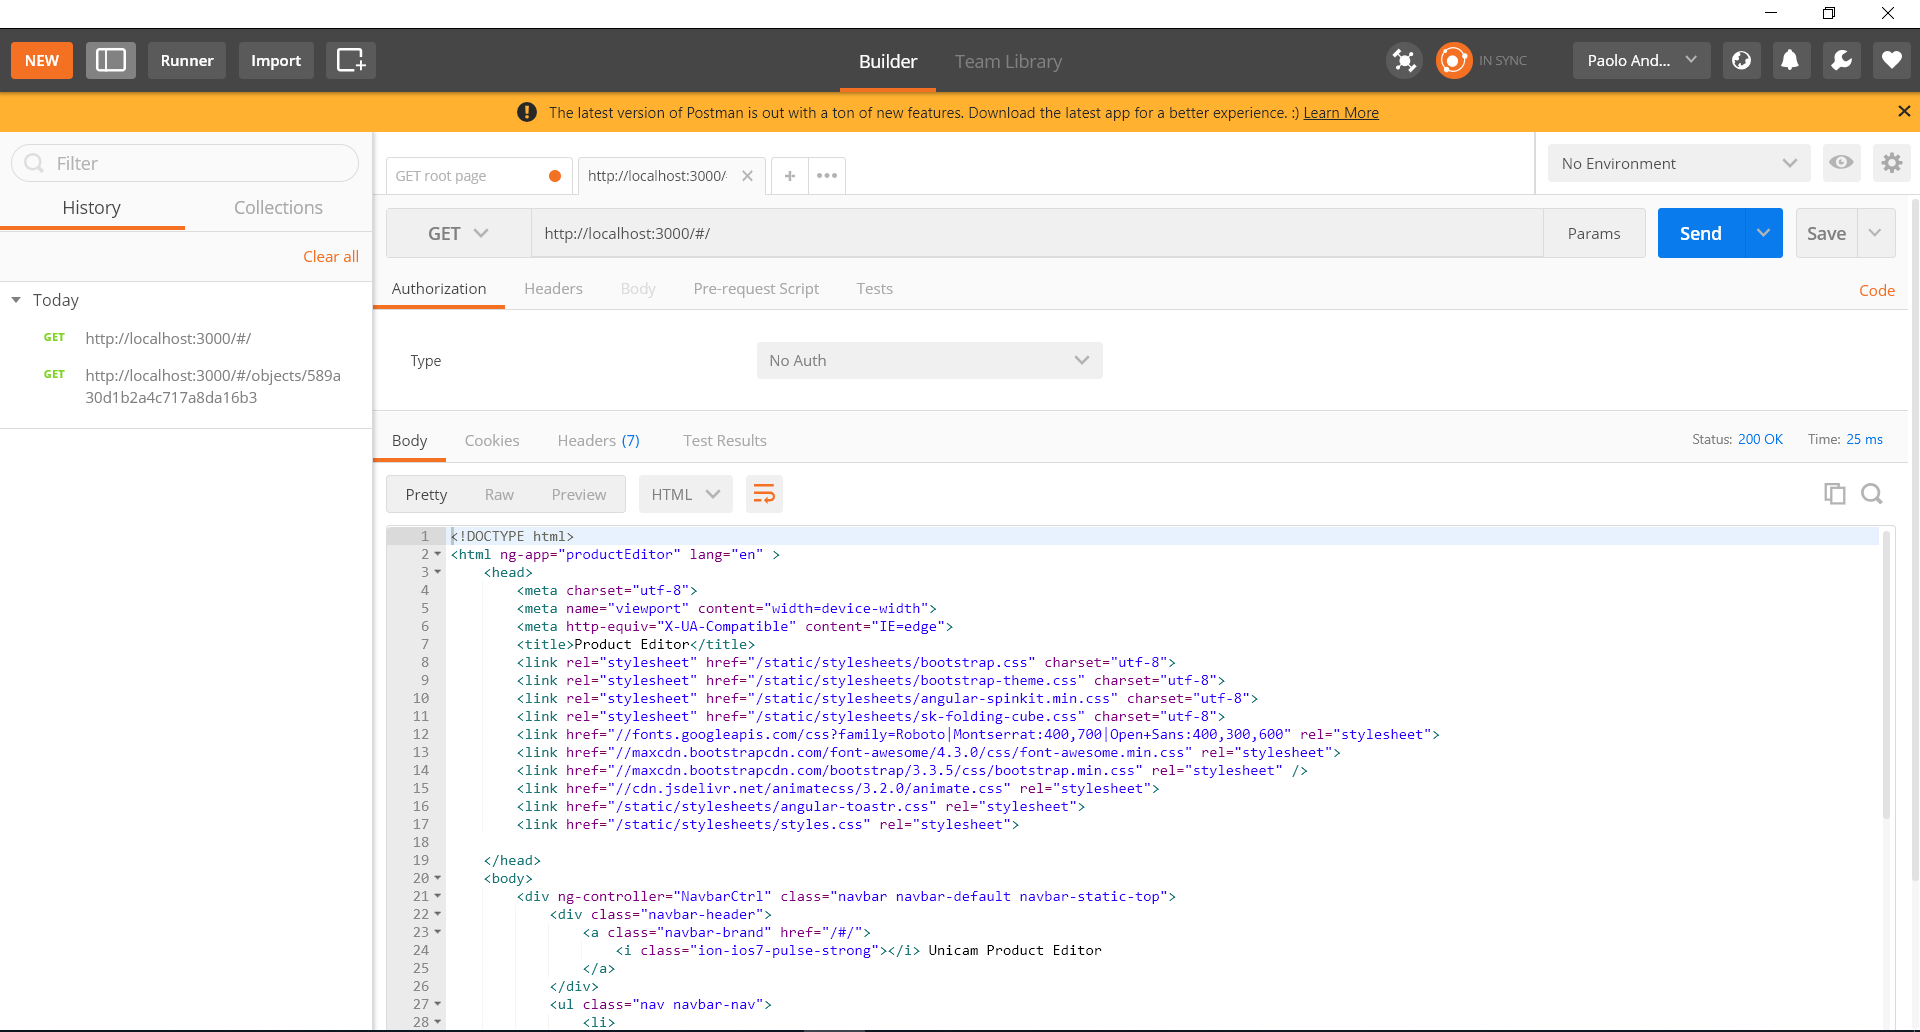
\includegraphics[scale=0.35]{Immagini/postman_ui.png}
	\caption{L'interfaccia utente di Postman}
\end{figure}

\section{NodeJS}
Node.js\cite{node}\index{Node} v4 è un interprete JavaScript orientato agli eventi, progettato per realizzare applicazioni di rete scalabili.
La caratteristica principale è che rimane inattivo finché non arriva una connessione in ingresso, o più generalmente un qualsiasi evento, e viene chiamata la relativa callback.
Questo paradigma è in contrasto con quello tradizionale basato sui thread.
Il principale vantaggio del paradigma ad eventi rispetto a quello basato sui thread si ha quando c'è un alto traffico.
In questo caso, infatti, l'alto numero di thread genera un alto overhead diminuendo drasticamente le prestazioni della macchina host.
Inoltre, dato che nessuna funzione di Node eseguirà direttamente operazioni di I/O, il processo non si bloccherà mai.

La versione di Node usata in unicam-product-editor è la v4.6.0.
Se da un lato su un server è normale avere solo una versione di Node, potrebbe non esserlo su una macchina di sviluppo.
Può capitare, infatti, che uno sviluppatore sia impegnato su più progetti Node che utilizzano versioni differenti.
Per risolvere questo problema possiamo installare NVM\index{NVM}.
Node Version Manager permette di avere più versioni di Node contemporaneamente nel nostro sistema e fornisce una semplice CLI per poterle gestire.
In particolare, basta creare un file di testo chiamato \texttt{.nvmrc} in cui salvare il numero di versione di Node che si intende usare per la cartella corrente.
Poi, sarà sufficiente digitare il comando \texttt{nvm install} per scaricare ed utilizzare la giusta versione.

Node è disponibile per diverse piattaforme, come Linux, Microsoft Windows e Apple OS X.
Le applicazioni Node.js vengono costruite utilizzando librerie e moduli disponibili per l'ecosistema ed alcuni di essi sono stati utilizzati in unicam-product-editor.
Per iniziare ad utilizzare Node.js, dobbiamo per prima cosa creare un file \texttt{package.json}, che descrive la nostra applicazione ed elenca tutte le sue dipendenze.
NPM (Node.js Package Manager)\index{NPM} installa una copia delle librerie in una sotto-cartella chiamata \texttt{node\_modules/}, della cartella principale dell'applicazione. 
Questo comporta diversi benefici, ad esempio isola le diverse versioni delle librerie, evitando così i problemi di compatibilità che si sarebbero presentati se avessimo installato tutto in una cartella standard come \texttt{/usr/lib}.

Il comando \texttt{npm install} creerà la cartella \texttt{node\_modules/}, con dentro tutte le librerie richieste e specificate nel file package.json:

\begin{lstlisting}[caption={package.json}, style=javaScriptCode][h]
{
	"name": "unicam-product-editor",
	"version": "1.0.0",
	"private": "true",
	"description": "Editor di prodotti 3D",
	"repository": "https://github.com/e-xtrategy/unicam-product-editor",
	"main": "app.js",
	"scripts": {
		"test": "nodemon --ignore tmp/ app.js",
		"start": "node app.js"
	},
	"author": "Paolo Andreassi",
	"license": "ISC",
	"dependencies": {
	...
	"async": "^2.1.4",
	"bcryptjs": "^2.4.0",
	"body-parser": "^1.15.2",
	...
	"cors": "^2.8.1",
	"express": "^4.14.0",
	"express-fileupload": "0.0.5",
	"express-handlebars": "^3.0.0",
	...
	"mongodb": "^2.2.10",
	"mongoose": "^4.7.8",
	...
	"python-shell": "^0.4.0",
	...
	"satellizer": "^0.15.5",
	...
	},
	"devDependencies": {
		"nodemon": "^1.11.0",
		"should": "~7.1.0",
		"supertest": "~1.1.0"
	},
		"engines": {
		"node": "4.6.0"
	}
}
\end{lstlisting}
\newpage
E' interessante analizzare alcune parti di questo file, oltre al fatto che anche questo è in formato JSON, e oltre alle prime righe che descrivono il progetto in sé per sé.
Ci sono due script: quello chiamato \emph{start} avvia l'applicazione normalmente tramite il comando \texttt{node} seguito dal nome del file principale del server \texttt{app.js}.
Lo script chiamato \emph{test} invece è interessante, perché avvia uno strumento (installato tramite l'apposita dipendenza) chiamato nodemon. Questo utilissimo \emph{demone} fa sì che in fase di test ogni qual volta si verifichi un errore che interrompe l'esecuzione del server nodemon attende un salvataggio dei file del progetto, che indica che lo sviluppatore ha modificato il codice per correggere l'errore, e non appena questo evento si verifica il demone riavvia in automatico il server ricominciando ad eseguire il codice.

Un'altra dipendenza interessante riguarda \emph{python-shell}, che nel nostro progetto servirà ad eseguire lo script della libreria Three.js scritto in codice Python (altrimenti non eseguibile da Javascript), che si occupa di convertire il file .obj in JSON. python-shell può ricevere in input interi file scritti in Python per eseguirli in modo asincrono.

Focalizziamoci ora sulla dipendenza \emph{async} per poter entrare nel dettaglio in una peculiarità di Node.js.
Qualsiasi operazione che ha a che fare con blocchi di I/O, come leggere un file o interrogare un database, prenderà una callback come ultimo parametro e continuerà l'esecuzione del programma, ma
solo quando l'operazione sarà completa il programma richiamerà la callback. Questo accade perché Node.js è progettato per eseguire le istruzioni in modo asincrono.

\begin{lstlisting}[caption={operazioni asincrone}, style=javaScriptCode, label={lst:async}]
function foo() {
	someAsyncFunction(params, function(err, results) {
		console.log("one");
	});
	console.log("two");
}
\end{lstlisting}

Dal codice \ref{lst:async} ci si potrebbe aspettare che il risultato sia:
\texttt{onetwo}.\\
In realtà potrebbe capitare che l’output sia \texttt{twoone}.

Questa caratteristica dei programmi asincroni è detta esecuzione non deterministica. Anche se permette al programma di essere particolarmente performante, si può avere la necessità in alcuni casi di eseguire delle determinate istruzioni prima di altre o in un certo ordine.

Per risolvere il problema della programmazione non deterministica si usa Async.
Async è un modulo che fornisce delle funzioni per lavorare con il JavaScript in modo asincrono, che seguono la convenzione di Node.js di mettere una singola callback come ultimo parametro della funzione. 
\newpage
L'esempio seguente illustra come stampare i due numeri nell'ordine corretto utilizzando la libreria async:

\begin{lstlisting}[caption={operazioni sincrone}, style=javaScriptCode]
actionArray = [
	function one(cb) {
		someAsyncFunction(params, function(err, results)  {
			if (err) {
				cb(new Error("There was an error"));
			}
			console.log("one");
			cb(null);
		});
	},
	function two(cb) {
		console.log("two");
		cb(null);
	}
]
async.series(actionArray);
\end{lstlisting}

Così facendo il risultato sarà quello aspettato, ossia \texttt{one} verrà stampato sicuramente prima di \texttt{two}.